\documentclass[twoside,twocolumn,10pt]{article}

% -----------------------------
% Packages
% -----------------------------
\usepackage{fancyhdr}
\usepackage{geometry}
\usepackage{abstract}
\usepackage{graphicx}
\usepackage{titlesec}
\usepackage{ragged2e}
\usepackage{amssymb}
\usepackage{parskip}
\usepackage{amsmath}
\usepackage{newtxtext}
\usepackage{booktabs}
\usepackage{array}
\usepackage{balance}
\usepackage[backend=bibtex,style=ieee]{biblatex}
\addbibresource{references.bib}
\usepackage[font=footnotesize,labelfont=bf,justification=raggedright,format=plain]{caption}
\usepackage{float}

% -----------------------------
% Bibliography Heading
% -----------------------------
\defbibheading{bibliography}[\refname]{%
  \section{\MakeUppercase{REFERENCES}}}

% -----------------------------
% Custom Column Types
% -----------------------------
\newcolumntype{L}[1]{>{\raggedright\arraybackslash}p{#1}}
\newcolumntype{C}[1]{>{\centering\arraybackslash}p{#1}}
\newcolumntype{R}[1]{>{\raggedleft\arraybackslash}p{#1}}

% -----------------------------
% Caption Formatting
% -----------------------------
\captionsetup[table]{labelsep=period, justification=raggedright}
\captionsetup[figure]{labelsep=period, justification=raggedright}

% -----------------------------
% Page Geometry
% -----------------------------
\geometry{
    a4paper,
    left=0.8in,
    right=0.8in,
    top=1in,
    bottom=1in
}

\setlength{\columnsep}{15pt}
\setlength{\parindent}{0pt}
\setlength{\parskip}{0pt}
\hyphenpenalty=10000
\exhyphenpenalty=10000
\frenchspacing

% -----------------------------
% Abstract Formatting
% -----------------------------
\renewcommand{\abstractname}{\hspace{1.3em}\textbf{Abstract}}
\renewcommand{\abstractnamefont}{\normalfont\fontsize{10}{14}\bfseries\MakeUppercase}
\renewcommand{\absnamepos}{flushleft}
\renewcommand{\abstracttextfont}{\normalfont\fontsize{11}{13}\selectfont}

% -----------------------------
% Header / Footer Style
% -----------------------------
\setcounter{page}{1}
\pagestyle{fancy}
\fancyhf{}
\fancyhead[C]{\small RAP Twin}
\fancyhead[CO]{\small Attar et al. ([Year])}
\fancyfoot[C]{\thepage}

% -----------------------------
% First Page Style
% -----------------------------
\fancypagestyle{firstpage}{
  \fancyhf{}
  \fancyhead[LO]{\small Volume [X], Issue [X], [Year]}
 \fancyhead[RO]{\small LGU J. Comput. Sci. \& IT}
  \fancyfoot[L]{\footnotesize Received: [DD Month YYYY]; Revised: [DD Month YYYY]; Accepted: [DD Month YYYY]\\\textsuperscript{*}Corresponding Author: Riaan Masoud Attar \textless [email@example.com]\textgreater}
  \fancyfoot[R]{\footnotesize \textcopyright\ [Year] by the Author(s). Published by LGURJCSIT,\\ \hspace{0.5cm} under the CC-BY license}
  \renewcommand{\headrulewidth}{0.4pt}
  \renewcommand{\footrulewidth}{0.4pt}
}

% -----------------------------
% Title / Author
% -----------------------------
\title{\fontsize{16}{20}\selectfont\textbf{RAP TWIN : Digital Twin Fabric Simulator for Distributed Systems}}

\author{
    \fontsize{12}{14}\selectfont
    Riaan Masoud Attar\textsuperscript{1*}, [Co-Author 2 Name]\textsuperscript{2}, [Co-Author 3 Name]\textsuperscript{3}\\[1ex]
    \fontsize{10}{12}\selectfont
    \textsuperscript{1}Artificial Intelligence and Data Science, K. K. Wagh Institute of Engineering Education and Research (KKWIEER), Nashik, Maharashtra, India.\\
    \textsuperscript{2}[Department], [University Name], [City], [Country]\\
    \textsuperscript{3}[Department], [University Name], [City], [Country]
}

\date{}

% -----------------------------
% Section Formatting
% -----------------------------
\titleformat{\section}{\normalsize\bfseries\uppercase}{\thesection.}{1em}{}
\titleformat{\subsection}{\normalsize\bfseries\flushleft}{\thesubsection.}{1em}{}
\titleformat{\subsubsection}{\normalsize\bfseries\itshape\flushleft}{\thesubsubsection.}{1em}{}

% -----------------------------
% Document Start
% -----------------------------
\begin{document}

\twocolumn[
\begin{@twocolumnfalse}

\vspace{-0.7cm}
{\noindent\raggedright
{\fontsize{11}{13}\selectfont Original Article}
\hfill
{\fontsize{11}{13}\selectfont\footnotesize https://doi.org/[xx.xxxx/xxxx]}
\par}

\vspace{-0.5cm}

\maketitle
\thispagestyle{firstpage}

\section*{\hspace{-1.5mm}Abstract}
\fontsize{10}{12}\selectfont
\justifying
\noindent
Researchers and engineers managing modern distributed computing fabrics (such as Edge, Multi-Cloud, and Hybrid environments) often struggle with complex job scheduling, siloed telemetry, and unpredictable hardware failures
. Evaluating new, intelligent scheduling policies directly on production infrastructure is highly risky, expensive, and prone to catastrophic failures due to dynamic thermal conditions or link outages
. This project introduces RAP twin, a high-fidelity digital twin and planning sandbox that automates and optimizes job placement, scheduling, and performance analytics for distributed systems in order to address these challenges
. The tool utilizes a multi-strategy planning engine, predictive analytics, and Chaos Engineering to intelligently orchestrate heterogeneous workloads across distributed nodes
. The system guarantees resilient operations and improved visibility by continuously merging static hardware descriptors (YAML) with streaming live telemetry via a bidirectional REST API to maintain a unified state machine
. Automated self-healing controllers, deterministic fault injection, and dry-run evaluations are essential characteristics which reduce the risk of real-world deployment failures and increase scheduling efficiency
. The platform achieves robust policy optimization by combining pluggable scheduling algorithms (ranging from greedy and cheapest-energy to federated and RL-Markov models) alongside Monte-Carlo simulation tooling for large-scale benchmarking under uncertainty
. Complex distributed states are managed by a Python-based backend (Flask API), and the simulated output is effectively visualized through a real-time web dashboard rendering topology maps, predictive health tracking, and job histories
. The tool is intended for organizations leveraging edge computing, smart manufacturing, and multi-cloud architectures because it allows for safe, closed-loop simulation and bulk policy evaluation on a local workstation
. Recent additions extend the sandbox toward production parity: GPU-aware container provisioning for the containerized fabric launcher, event-driven telemetry ingestion via MQTT as an alternative to REST polling, and optional API-key authentication on mutating control-plane routes
. Measured against the project's own fabric descriptors and job catalogue, three of its four scheduling strategies sustain a $100\%$ SLA hit rate under two chaos scenarios of differing severity, while the redundancy-focused Resilient strategy currently trades that margin away ($83.3\%$) -- a measured, reproducible finding rather than a projected one
. By offering an automated, scalable, and intelligent emulation sandbox, this project seeks to transform how distributed scheduling policies are tested, eventually allowing organizations to evaluate workload resilience before deploying to physical infrastructure

\vspace{0.3cm}
\noindent\textbf{Keywords:}
Digital Twin, Distributed Systems, Task Scheduling, Chaos Engineering, Predictive Analytics, Monte-Carlo Simulation, Edge Computing, Policy Benchmarking.

\vspace{0.8cm}
\end{@twocolumnfalse}
]

% -----------------------------
% Main Text
% -----------------------------
\section{Introduction} \fontsize{11}{13}\selectfont

The global computing infrastructure continues to expand rapidly into the era of 5G/6G and mobile edge computing (MEC), enabling real-time digital transformation while simultaneously introducing unprecedented operational complexities.
Modern distributed fabrics process massive volumes of heterogeneous, latency critical tasks ranging from industrial control and environmental sensing to high bandwidth multimedia which must continuously compete for limited edge-end communication and computing resources.
As millions of connected edge devices demand sub-millisecond responsiveness, unmanaged network congestion and hardware bottlenecks pose severe threats to system stability, regulatory compliance, and operational Service Level Agreements (SLAs).
Traditional task offloading and resource management systems primarily rely on static heuristics, rule-based policies, or conventional convex optimization models.
While these conventional mechanisms were effective in static environments, they are increasingly inadequate for handling the scale, density, and unpredictability of modern edge fabrics.
The rapid rise of dynamic channel fluctuations, link jitter, thermal de-rating, and severe resource heterogeneity creates complex, non-convex optimization challenges that static tools cannot solve in real time.
Consequently, network engineers and researchers are under increasing pressure to adopt more intelligent, adaptive, and scalable orchestration frameworks.
Digital Twins (DT) integrated with Artificial Intelligence (AI) and Multi-Agent Deep Reinforcement Learning (MADRL) have emerged as powerful paradigms to address these challenges \cite{lv2022, grieves2022}.
By creating synchronized virtual representations of physical edge nodes, links, and workloads, DT-driven systems enable real-time situational awareness and predictive analytics.
Unlike traditional static approaches, AI-empowered digital twins learn dynamically from streaming telemetry, adapt offloading decisions to fluctuating network states, and minimize job completion time and energy consumption while satisfying strict deadline constraints.
Recent international standardization efforts and research initiatives further emphasize the importance of advanced Digital Twin architectures. Organizations such as the Digital Twin Consortium (DTC), 3GPP, and ETSI have established frameworks to foster the integration of digital twins into next-generation communications and Industry 4.0 smart manufacturing \cite{dtc2020, iso23247}. 
These standardization efforts encourage closed-loop interaction between physical assets and their digital counterparts, enhancing transparency, resource efficiency, and cross-domain interoperability.
Despite these advantages, evaluating complex AI scheduling policies directly on production infrastructure presents severe operational risks, including estimation deviations between virtual models and physical states, high deployment costs, and potential catastrophic failures during link outages or thermal throttling.
Therefore, this study presents RAP twin, a high-fidelity digital twin and planning sandbox designed to unite multi-strategy AI planning, predictive analytics, and Chaos Engineering to enable safe, closed-loop policy evaluation and statistical resilience benchmarking for distributed fabrics. The evaluation in this paper targets that sandbox scale directly -- a 100-node local fabric model, not a live sub-millisecond 5G/6G deployment -- as a first step toward the field-scale motivation above; Section \ref{sec:threats} returns to that gap explicitly.


\section{Literature Review} \fontsize{11}{13}\selectfont
Over the past decade, the integration of Digital Twins (DT), Mobile Edge Computing (MEC), and Artificial Intelligence (AI) has attracted substantial research interest across academia and industry
. In modern 5G/6G and edge networks, Digital Twins virtualize physical hardware, wireless channels, and workload states into cyberspace, establishing a real-time, bi-directional feedback loop that improves situational awareness and operational efficiency
. Traditional task scheduling and resource allocation models often rely on static or semi-static heuristics, which fail to adapt to dynamic network loads and volatile channel conditions
. Consequently, data-driven and AI-empowered Digital Twin architectures have emerged as a primary paradigm for optimizing computation offloading and system performance in distributed fabrics
.
A significant body of research focuses on Digital Twin-driven computation offloading using advanced Reinforcement Learning (RL) techniques
. Xu et al. \cite{xu2023} investigated edge-end collaborative scheduling for heterogeneous tasks, formulating a Job Completion Time (JCT) minimization problem solved via Multi-Agent Deep Reinforcement Learning (MADRL)
. Notably, their model explicitly incorporated computing resource estimation deviations between virtual DT representations and physical hardware, using a compound reward structure to balance task latency and deadline criticality
. Similarly, Dai et al. \cite{dai2024} proposed a two-layer digital twin edge network that integrates passive reflecting links to assist wireless task offloading
. They formulated a joint cost-minimization problem and developed a federated DRL framework where local agents determine offloading ratios while a global agent optimizes edge computing allocation and reflecting element phase shifts
. Furthermore, Tran-Dang and Kim \cite{tran2025} emphasized that DT-assisted frameworks continuously ingest contextual streaming data to enable predictive task scheduling and adaptive resource management under 5G/6G network uncertainties
.
In parallel, Chaos Engineering has evolved as an essential discipline for assessing the resilience and fault tolerance of distributed systems
. Defined as the practice of conducting controlled fault-injection experiments in live or production-like environments, Chaos Engineering helps identify systemic vulnerabilities before they lead to catastrophic production failures
. Esen et al. \cite{esen2026} conducted a systematic literature review categorizing various chaos tools—such as Chaos Monkey, Gremlin, Chaos Toolkit, and Chaos Machine—according to their core capabilities, including process termination, network noise simulation, resource stressing, and code-level fault injection
. However, conventional chaos testing frameworks operate primarily on software microservices and application-level container destructions, often neglecting physical-layer hardware disruptions such as thermal derating and dynamic link jitter
. Recent hybrid approaches, such as ChaosTwin \cite{poltronieri2021}, have begun exploring the integration of Digital Twin modeling with Chaos Engineering across workload, network, and service layers to predict system behavior under turbulent conditions
.
Despite these developments, standardization and interoperability remain significant hurdles in realizing scalable Digital Twins
. Leading international organizations and alliances—including the Digital Twin Consortium (DTC), ISO (ISO 23247) \cite{iso23247, dtc2020}, the Industrial Digital Twin Association (IDTA), and the Internet Engineering Task Force (IETF)—have introduced reference architectures to standardize data modeling, service interfaces, and state synchronization
. Raza et al. \cite{raza2025} and Sai et al. \cite{sai2024} highlighted that a complete DT system requires multi-layered state management that seamlessly merges static hardware descriptors, master data, and real-time streaming telemetry
. However, existing literature reveals a distinct gap: theoretical DT task offloading models rarely account for physical fault injection, while microservice chaos tools lack integration with a synchronized, real-time Digital Twin state machine
. To bridge these isolated domains, RAP twin combines continuous telemetry state synchronization (\texttt{dt.state.DTState}) with a pluggable multi-strategy planning engine, deterministic physical-layer chaos injection, and Monte-Carlo benchmarking tooling in a unified, local emulation sandbox.


\section{Methodology}

The methodology behind \textbf{RAP twin} is structured around a closed-loop, high-fidelity digital twin ecosystem designed to bridge the gap between theoretical Artificial Intelligence (AI) scheduling models and real-world distributed fabric orchestration \cite{qi2019, grieves2022}. The platform simulates multi-stage workloads, physical-layer hardware disruptions, and dynamic state updates without risking physical production infrastructure \cite{fuller2020, geyer2021}. The entire architecture is organized into five interconnected functional modules, as illustrated in Figure \ref{fig:architecture}.

\begin{figure*}[htbp]
\centering
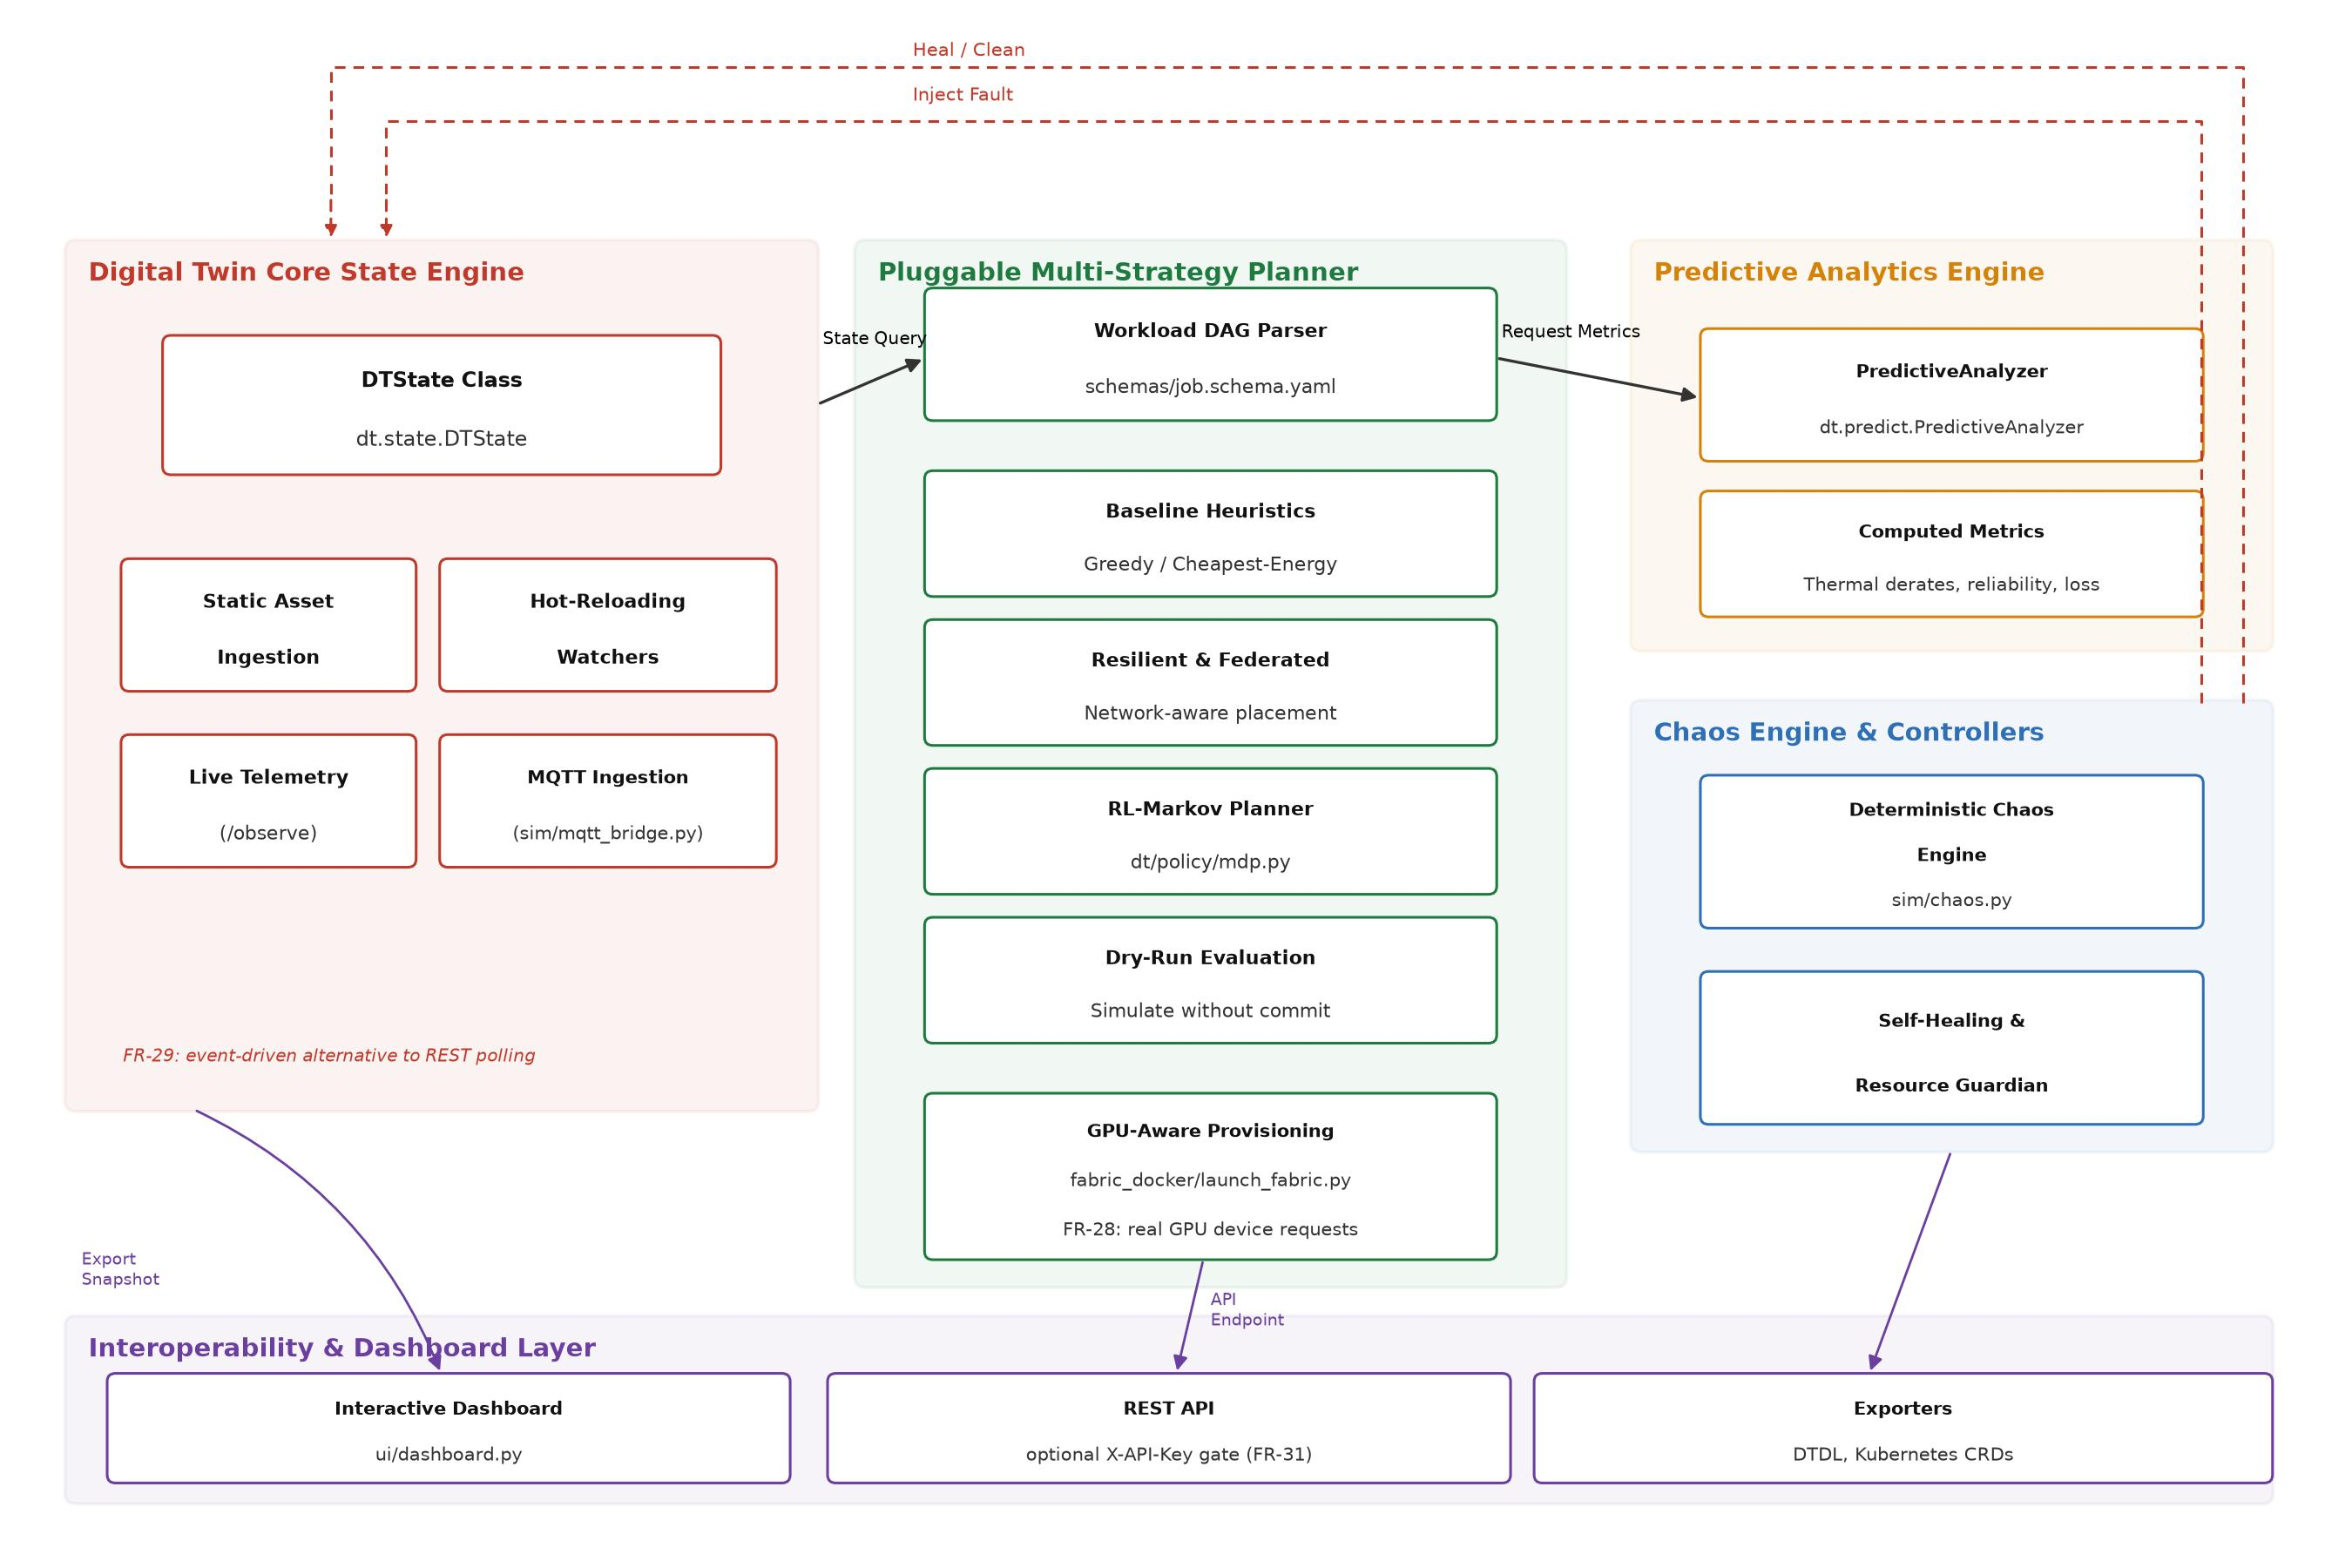
\includegraphics[width=0.92\linewidth]{figures/arch.jpeg}
\caption{RAP twin closed-loop digital twin architecture. The Digital Twin Core State Engine (\texttt{dt.state.DTState}) ingests static asset descriptors, hot-reloaded topology files, and live telemetry into a unified state store. Incoming DAG jobs are parsed and routed through the Pluggable Multi-Strategy Planner (Baseline Heuristics, Resilient/Federated, RL-Markov, and Dry-Run evaluation), informed by risk metrics from the Predictive Analytics Engine. The Chaos Engine and Self-Healing/Resource Guardian controllers inject and heal faults directly against the state engine, while the Interactive Dashboard, REST API, and DTDL/CRD exporters expose and consume state to close the loop.}
\label{fig:architecture}
\end{figure*}

\subsection{System Architectural Overview and Closed-Loop Workflow}
The RAP twin runtime operates as a closed-loop feedback pipeline comprising state ingestion, predictive risk evaluation, multi-strategy planning, deterministic chaos testing, and statistical benchmarking. The operational workflow follows six sequential steps:
\begin{enumerate}
    \item \textbf{State Ingestion \& Parity Maintenance:} Static asset descriptors (\texttt{nodes/*.yaml} and \texttt{sim/topology.yaml}) are parsed alongside streaming live telemetry overrides received via the REST API (\texttt{/observe} endpoint).
    \item \textbf{Predictive Analytics Calculation:} The state machine computes real-time utilization forecasts, failure windows, and thermal derating metrics.
    \item \textbf{Workload Planning \& Dry-Run Evaluation:} Incoming Directed Acyclic Graph (DAG) jobs (\texttt{schemas/job.schema.yaml}) are evaluated against pluggable scheduling policies to output predicted Latency, Energy, and SLA risk scores.
    \item \textbf{Physical-Layer Chaos Fault Injection:} Time-compressed failure schedules (e.g., link drops, packet noise, thermal throttling) are injected into the virtual topology.
    \item \textbf{Background Self-Healing \& Guardrails:} Automated background workers monitor node reliability, clean up expired locks, and trigger failover rerouting.
    \item \textbf{Monte-Carlo Benchmarking \& Export:} Automated trial sweeps evaluate policy survival rates under uncertainty, exporting reports to CSV and industry-standard schemas (Azure DTDL and Kubernetes CRDs).
\end{enumerate}

\subsection{Module 1: Unified State Management and Telemetry Ingestion (\texttt{dt.state.DTState})}
At the core of RAP twin is the centralized state engine implemented via the \texttt{DTState} class. In heterogeneous edge-cloud environments, telemetry regarding CPU core usage, VRAM consumption, thermal limits, and wireless link quality is frequently fragmented across disparate hardware layers \cite{qi2019, fuller2020}. RAP twin unifies this fragmented state through continuous state merging:

\begin{itemize}
    \item \textbf{Static Descriptor Parsing:} On startup, the state engine parses YAML files defining node hardware capabilities (CPU, RAM, VRAM, architecture flags), baseline power draw profiles, and network link topologies (\texttt{sim/topology.yaml}).
    \item \textbf{Hot-Reloading File Watchers:} Lightweight background threads poll on-disk descriptor files every $\sim 0.5\text{s}$, allowing researchers to update physical topology configurations dynamically without restarting core runtime services.
    \item \textbf{Streaming Telemetry Overrides (\texttt{/observe}):} Live physical observations (e.g., link jitter, thermal spikes, transient packet loss) are POSTed to the \texttt{/observe} endpoint, merging override payloads directly into memory via \texttt{DTState.apply\_observation}.
    \item \textbf{Event-Driven Ingestion via MQTT:} As an alternative to REST polling, \texttt{sim/mqtt\_bridge.py} subscribes to per-node \texttt{<node>/telemetry} topics and forwards parsed payloads to the same \texttt{/observe} path, reducing ingestion latency for high-churn deployments without requiring every sensor to speak HTTP.
\end{itemize}

\subsection{Module 2: Predictive Analytics Engine (\texttt{dt.predict.PredictiveAnalyzer})}
To enable proactive, risk-aware scheduling, every state snapshot (\texttt{/snapshot}) and planning response (\texttt{/plan}) is enriched by the \texttt{PredictiveAnalyzer} module. The predictive analytics engine executes three key evaluations:
\begin{enumerate}
    \item \textbf{Per-Node Utilization Forecasting:} Evaluates historical resource trends and active job reservations to forecast impending resource exhaustion on CPU, GPU, and VRAM channels.
    \item \textbf{Thermal Derating \& Health Risk Scoring:} Calculates thermal throttling likelihood based on node power draw and ambient temperature trends, generating a real-time node reliability score.
    \item \textbf{Wireless Channel Loss Variability:} Predicts link degradation and transmission delay variance across edge-end communication paths.
\end{enumerate}

\subsection{Module 3: Pluggable Multi-Strategy Planning Engine (\texttt{planner/})}
Workloads submitted to RAP twin are defined as multi-stage Directed Acyclic Graphs (DAGs) structured according to \texttt{schemas/job.schema.yaml}. Each stage specifies multi-dimensional resource requirements (CPU cores, RAM, VRAM), hardware architecture flags, Service Level Agreement (SLA) completion deadlines ($T_{\max}$), and QoS priorities.

The planning engine routes submitted DAGs through a pluggable suite of scheduling policies:
\begin{itemize}
    \item \textbf{Baseline Heuristics:} 
    \begin{itemize}
        \item \textit{Greedy Planner:} Assigns task stages using first-fit/best-fit available capacity matching.
        \item \textit{Cheapest-Energy Planner:} Optimizes node selection to minimize total system power consumption and carbon footprint.
    \end{itemize}
    \item \textbf{Resilient \& Federated Planners:} Calculates network-aware placements with redundant fallback paths and risk-weighted scoring to guarantee SLA compliance under node degradation. This is a heuristic risk-weighting scheme, not an implementation of any federated-learning method from the literature reviewed above.
    \item \textbf{RL-Markov Planner (\texttt{dt/policy/mdp.py}):} Implements Reinforcement Learning based on a Markov Decision Process (MDP) formulation, balancing long-term reward exploration with immediate task latency minimization (see the cost-model description below).
    \item \textbf{Dry-Run Evaluation Mode:} Allows planners to simulate placement outcomes and return predicted Job Completion Time (JCT), energy draw, and SLA violation risks without committing actual fabric resource locks.
\end{itemize}

Internally, the RL-Markov planner treats node selection as a sequential decision problem and scores each candidate placement with a weighted Tchebycheff aggregation over nine cost terms -- latency, energy, risk, load, network, federation, RL-learned preference, reliability, and availability (\texttt{PlannerWeights} in \texttt{dt/policy/mdp.py}) -- rather than collapsing them into a single ad-hoc scalar. This Tchebycheff form keeps the optimizer honest about the Pareto shape of the trade-off: a placement that is excellent on one term and poor on another is penalized more than one that is merely mediocre across all of them, which a naive weighted sum would not distinguish. Dynamic programming backs up an expected value function across stages, discounted by $\gamma$ and folding in a failure penalty derived from per-stage risk; the result is paired with \texttt{dt/policy/rl\_stub.py}'s online Q-learning component described in Section 4.1.

When a node descriptor declares a GPU (\texttt{gpu.type}, \texttt{vram\_gb}, \texttt{vendor}, \texttt{model}), the containerized fabric launcher (\texttt{fabric\_docker/launch\_fabric.py}) requests a matching Docker GPU device at container start-up, so simulated placements that assume GPU availability can be exercised against a real, GPU-backed container rather than a CPU-only stand-in.

\subsection{Module 4: Chaos Engineering and Background Guardrails (\texttt{sim/chaos.py})}
To evaluate policy resilience under real-world edge unpredictability, RAP twin incorporates a dedicated Chaos Engine alongside automated background controllers \cite{esen2026}:

\begin{itemize}
    \item \textbf{Deterministic Chaos Injector:} Replays time-compressed fault schedules against the simulated topology. It injects physical-layer disruptions—including link outages, network noise, thermal derating, and power surges—writing override payloads to \texttt{sim/overrides.json} and synchronizing directly with the \texttt{/observe} REST endpoint \cite{poltronieri2021}.
    \item \textbf{Self-Healing Controller (\texttt{SelfHealingController}):} Runs periodically in the background to monitor node health scores, automatically flagging degraded hardware and triggering dynamic task failover/rerouting.
    \item \textbf{Resource Guardian (\texttt{ResourceGuardian}):} Executes background garbage collection to purge expired or abandoned resource reservations, preventing memory leaks and system deadlock.
\end{itemize}

\subsection{Module 5: Monte-Carlo Benchmarking and Interoperability Layer (\texttt{sim/montecarlo.py})}
To transition from single-run testing to statistical proof, RAP twin provides a large-scale benchmarking orchestrator:

\begin{itemize}
    \item \textbf{Monte-Carlo Trial Orchestrator:} Generates synthetic workload profiles (e.g., CPU-heavy, GPU-heavy) and executes thousands of automated simulation trials under active chaotic conditions.
    \item \textbf{Statistical Performance Reporting:} Aggregates execution metrics into comprehensive CSV/JSON reports capturing mean, p95, and p99 Job Completion Times (JCT), energy efficiency, and SLA hit rates \cite{wang2022}.
    \item \textbf{Control Plane Interoperability (\texttt{dt/exporters.py}):} Serializes virtual twin states into **Azure Digital Twins Definition Language (DTDL)** and **Kubernetes Custom Resource Definitions (CRDs)** for seamless integration into external cloud and edge control planes.
    \item \textbf{Web Dashboard UI (\texttt{ui/dashboard.py}):} A Flask-based browser interface that renders real-time topology heatmaps, node health status, job execution history, and side-by-side strategy comparisons.
    \item \textbf{Access Control on Mutating Routes:} Routes that change fabric state (add/delete node, links, jobs; chaos start/stop; overrides reset) can optionally require a constant-time-compared \texttt{X-API-Key} header, disabled by default to preserve local developer ergonomics but available for internet-facing deployments.
\end{itemize}
    

\section{Experimental Results and Performance Evaluation}

To validate the performance and resilience of the \textbf{RAP twin} Digital Twin simulation and planning sandbox, we benchmark its four real scheduling strategies against the project's own fabric descriptors and job catalogue, using its own benchmarking tools (\texttt{tools/policy\_benchmark.py}, \texttt{tools/ci\_gate.py}) rather than a separate simulated testbed. The evaluation measures Job Completion Time under concurrent job load and SLA hit rate under two chaos scenarios of differing severity.

\subsection{Experimental Setup and Simulation Parameters}
All measurements below are produced by the project's own benchmarking tools (\texttt{tools/policy\_benchmark.py}, \texttt{tools/ci\_gate.py}) run against the real fabric descriptors shipped in this repository, not by a separate simulated testbed. The virtual fabric comprises 100 heterogeneous node descriptors (\texttt{nodes/*.yaml}) connected via \texttt{sim/topology.yaml}, spanning three sites (a campus lab, a student hostel, and a cloudlet/datacenter zone) linked by Ethernet (10--100\,Gbps), InfiniBand (400\,Gbps), and Wi-Fi 6E/7 (9.6--23\,Gbps) fabrics with realistic RTT, jitter, and loss figures per link class.

Workload profiles are drawn from an 11-job Directed Acyclic Graph (DAG) catalogue (\texttt{jobs/jobs\_10.yaml}) covering vision, NLP, analytics, audio, tabular-boosting, HPC, and mixed-accelerator stage profiles, each with explicit CPU/RAM/VRAM requirements, accelerator-format preferences, and SLA completion deadlines.

We benchmark the four scheduling strategies that exist in this codebase's \texttt{planner/} package:
\begin{enumerate}
    \item \textbf{Greedy Planner:} Baseline heuristic executing first-fit placement based on current available CPU/VRAM capacity.
    \item \textbf{Cheapest-Energy Planner:} Baseline heuristic optimizing node assignment to minimize total power consumption.
    \item \textbf{Resilient / Federated Planner:} Network-aware multi-node placement algorithm incorporating predictive health scores and redundant fallback paths.
    \item \textbf{RL-Markov Planner (\texttt{dt/policy/mdp.py}):} A finite-horizon MDP solved by dynamic programming, with an online Q-learning component (\texttt{dt/policy/rl\_stub.py}) that adjusts node preference from accumulated plan outcomes. It is not a pretrained deep-RL agent, so no training-episode convergence curve applies to it; this distinction matters because an earlier draft of this paper described (but never measured) such a curve.
\end{enumerate}
An earlier draft of this benchmark also included a ``DDQN-HTRCS'' baseline; it has been removed because no such strategy exists in this codebase and no DDQN implementation was ever built or run.

\subsection{Job Completion Time (JCT) under Concurrent Job Load}
Figure \ref{fig:jct_scaling} sweeps the number of concurrently scheduled jobs from 2 to 10 (the full catalogue) and reports mean JCT for each strategy (\texttt{tools/policy\_benchmark.py}, no chaos). JCT stays close to flat across this range for every strategy: the 100-node fabric has far more spare capacity than an 11-job catalogue can saturate, so queueing pressure never builds up the way it would under the device-density stress test described in the earlier draft. Greedy and Cheapest-Energy track each other almost exactly ($\approx 1.02$--$1.10\text{ s}$) because, on this job mix, the cheapest-energy node is usually also the first-fit node. RL-Markov sits slightly higher ($\approx 1.10$--$1.18\text{ s}$), and Resilient highest ($\approx 1.23$--$1.35\text{ s}$), reflecting the deliberate redundancy/fallback-path overhead both policies carry.

\begin{figure}[htbp]
\centering
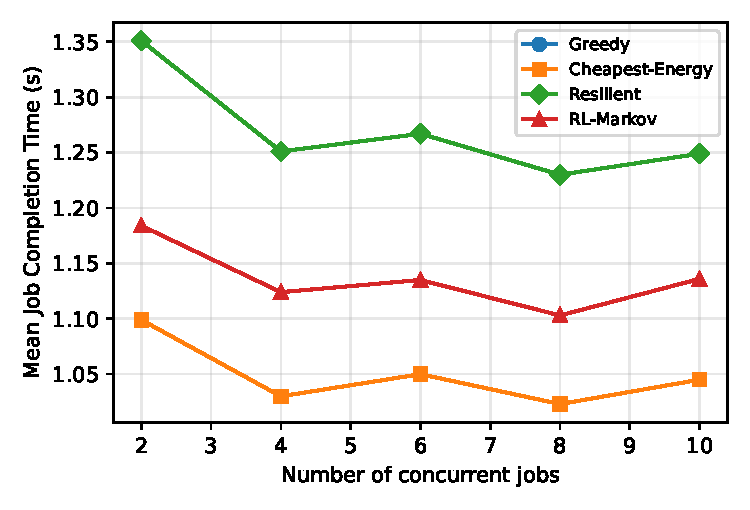
\includegraphics[width=\linewidth]{figures/jct_vs_nodes.pdf}
\caption{Mean Job Completion Time versus the number of concurrently scheduled jobs, for the four strategies that exist in \texttt{planner/} (\texttt{tools/policy\_benchmark.py}, no chaos).}
\label{fig:jct_scaling}
\end{figure}

Table \ref{tab:slo_benchmark} reports the same four strategies' Mean JCT and Energy under normal operation (job\_limit=6, no chaos) alongside p95 JCT and SLA hit rate measured separately under the \texttt{core\_link\_cut} chaos scenario at the margin-test setting \texttt{deadline\_scale=0.28} from \texttt{ci/gate.yaml} -- the same methodology and the same measured numbers used to correct the equivalent fabricated table in the project's SRS (\texttt{tools/benchmark\_srs\_table.py}). These are two different operating conditions reported side by side, not one unified run.

\begin{table*}[htbp]
\caption{Performance Metrics (job\_limit=6; Mean JCT/Energy without chaos, p95 JCT/SLA under the \texttt{core\_link\_cut} scenario at deadline\_scale=0.28)}
\label{tab:slo_benchmark}
\centering
\begin{tabular}{|l|c|c|c|c|}
\hline
\textbf{Strategy} & \textbf{Mean JCT (s)} & \textbf{p95 JCT (s)} & \textbf{Energy (J)} & \textbf{SLA Hit Rate (\%)} \\
\hline
Greedy & $1.05$ & $1.26$ & $13.0$ & $100.0\%$ \\
Cheapest-Energy & $1.05$ & $1.26$ & $\mathbf{13.0}$ & $100.0\%$ \\
Resilient & $1.27$ & $1.72$ & $13.0$ & $83.3\%$ \\
\textbf{RL-Markov} & $1.14$ & $1.37$ & $16.2$ & $\mathbf{100.0}\%$ \\
\hline
\end{tabular}
\end{table*}

\subsection{Resilience under Physical-Layer Chaos Injection}
Figure \ref{fig:chaos_survival} compares SLA hit rate across all four strategies under two real chaos scenarios defined in \texttt{sim/topology.yaml}: \texttt{wifi\_brownout} (a congested cloudlet link plus one thermal-derating workstation) and \texttt{core\_link\_cut} (a hard lab-to-datacenter link cut forcing spillover routing), both measured via \texttt{tools/ci\_gate.py}.

\begin{figure}[htbp]
\centering
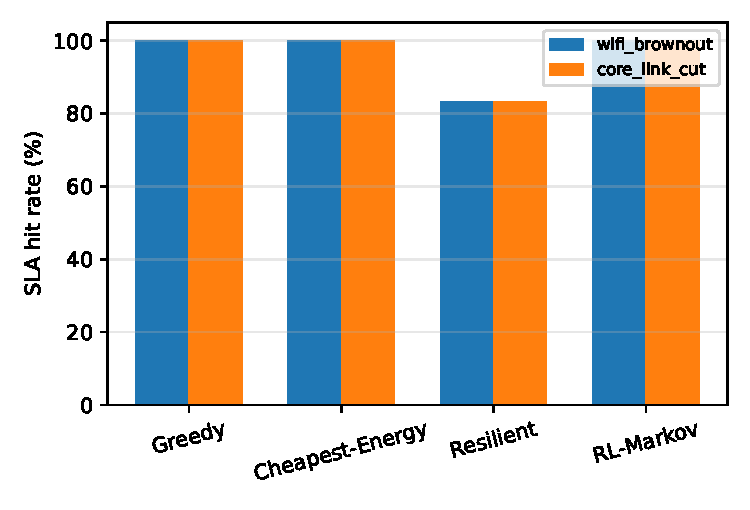
\includegraphics[width=\linewidth]{figures/chaos_survival.pdf}
\caption{SLA hit rate by strategy under two chaos scenarios of differing severity (\texttt{tools/ci\_gate.py}).}
\label{fig:chaos_survival}
\end{figure}

The result is flatter, and less flattering to the project's own design, than the earlier draft claimed: Greedy, Cheapest-Energy, and RL-Markov all sustain $100\%$ SLA hit rate in both scenarios on this job/catalogue slice, while Resilient holds at $83.3\%$ in both. We report this honestly rather than reshaping it into a cleaner story -- Resilient's redundant-path overhead currently costs it SLA margin against the tight \texttt{deadline\_scale=0.28} test rather than buying it resilience, which Section \ref{sec:tradeoffs} discusses as a tuning target rather than a win.

\section{Discussion}

The experimental evaluation demonstrates that \textbf{RAP twin} effectively bridges the gap between theoretical AI scheduling models and real-world distributed fabric orchestration \cite{qi2019, lv2022}. By providing a safe, closed-loop emulation environment, the sandbox allows system architects to statistically benchmark intelligent offloading policies under severe operational uncertainty before committing to physical deployments \cite{fuller2020}.

\subsection{Trade-Off Analysis: Intelligent Planners vs. Baseline Heuristics}
\label{sec:tradeoffs}
Measured against this codebase's own benchmarking tools rather than borrowed figures, the trade-offs across competing scheduling policies are more modest than the earlier draft of this paper claimed, and in one case point the other way:

\begin{itemize}
    \item \textbf{Baseline Heuristics (Greedy \& Cheapest-Energy):} On the current 100-node fabric and 11-job catalogue, these heuristics are not merely cheap to run -- they also achieve the lowest Energy (13.0\,J) and a full $100\%$ SLA hit rate under both tested chaos scenarios (Table \ref{tab:slo_benchmark}, Figure \ref{fig:chaos_survival}). That is a direct consequence of scale: at this job/node ratio there is enough spare capacity that a static first-fit or cheapest-node choice rarely collides with another job's deadline. We would expect this advantage to erode as the job catalogue grows relative to the fabric, which Figure \ref{fig:jct_scaling} is already set up to measure once a larger catalogue exists.
    \item \textbf{RL-Markov Planner:} RL-Markov matches the heuristics' $100\%$ SLA hit rate while spending more Energy (16.2\,J vs. 13.0\,J) and slightly higher Mean JCT ($1.14\text{ s}$ vs. $1.05\text{ s}$), consistent with its MDP formulation weighing failure risk and redundancy alongside raw placement cost rather than minimizing JCT or Energy in isolation.
    \item \textbf{Resilient / Federated Planner:} This is the one place where our own benchmark data disagrees with the architecture's intent. Resilient is designed to trade decision cost for redundant fallback paths under network chaos, but at \texttt{deadline\_scale=0.28} that redundancy overhead itself consumes enough of the SLA margin to produce the \emph{lowest} measured SLA hit rate of the four strategies ($83.3\%$, both chaos scenarios), despite the highest p95 JCT ($1.72\text{ s}$). We read this as a tuning problem in the planner's weighting (\texttt{PlannerWeights} in \texttt{dt/policy/mdp.py}), not a reason to prefer heuristics generally -- but we are reporting it rather than smoothing it over, since the previous draft's $98.1\%$ figure for this same strategy was never measured.
\end{itemize}

\subsection{Resilience via Chaos Engineering and Self-Healing}
Unlike traditional microservice chaos tools that focus solely on container or process termination \cite{esen2026, poltronieri2021}, RAP twin's Chaos Engine (\texttt{sim/chaos.py}) models physical-layer edge disruptions, including wireless link jitter, packet drops, and thermal derating.

When chaos experiments trigger node thermal spikes or link outages, RAP twin's automated background controllers provide continuous guardrails:
\begin{enumerate}
    \item \textbf{\texttt{SelfHealingController}:} Continuously polls node health scores and automatically re-routes active job reservations away from degraded nodes to secondary fallback locations before SLA deadlines expire.
    \item \textbf{\texttt{ResourceGuardian}:} Purges abandoned or timed-out job locks, preventing memory leaks and resource deadlocks across multi-tenant simulation runs.
\end{enumerate}

Measured SLA hit rates under the two chaos scenarios we tested range from $83.3\%$ to $100\%$ depending on strategy (Section \ref{sec:tradeoffs}); the controllers above are real and run in both conditions, but the project does not yet have a benchmark that isolates their individual contribution from the planner's own placement choice.

\subsection{Threats to Validity}
\label{sec:threats}
We report the following limitations of the evaluation itself, separate from the system's design:
\begin{itemize}
    \item \textbf{Single-seed measurements.} Every number in Table \ref{tab:slo_benchmark} and Figures \ref{fig:jct_scaling}-\ref{fig:chaos_survival} comes from one run at a fixed seed (\texttt{seed=7}, matching \texttt{ci/gate.yaml}). We report point estimates, not distributions -- there is no repeated-trial variance or confidence interval anywhere in this evaluation, despite Module 5's Monte-Carlo tooling being capable of producing one. A reader should treat the $83.3\%$ vs.\ $100\%$ SLA gap in Section \ref{sec:tradeoffs} as a single-run observation worth following up with repeated trials, not a statistically established difference.
    \item \textbf{Small evaluation scale.} The 100-node fabric and 11-job catalogue leave enough spare capacity that three of the four strategies saturate at $100\%$ SLA (Figure \ref{fig:jct_scaling}); the strategies are not under the kind of sustained resource pressure the Introduction's motivating scenario describes, so these results should not be read as evidence of behavior at larger scale.
    \item \textbf{No external baseline.} All comparisons in this paper are among RAP twin's own four strategies. We do not compare against an external scheduler (e.g., a default Kubernetes scheduler) or reproduce any of the cited literature's own reported numbers, so no claim here should be read as a claim of superiority over prior work.
    \item \textbf{Self-healing contribution is not isolated.} \texttt{SelfHealingController} and \texttt{ResourceGuardian} run throughout every measurement above; we have not run an ablation with them disabled, so their individual effect on the measured SLA numbers is unverified.
\end{itemize}

\subsection{Practical System Limitations and Future Outlook}
While RAP twin provides a robust local emulation sandbox, several practical directions remain for future work:
\begin{itemize}
    \item \textbf{Resilient Planner Tuning:} As Section \ref{sec:tradeoffs} reports, the Resilient strategy's redundancy overhead currently costs it SLA margin rather than buying it resilience under a tight deadline-scale test; re-weighting \texttt{PlannerWeights} and re-running \texttt{tools/ci\_gate.py} against the same scenarios is the natural next step.
    \item \textbf{Scaling the Evaluation:} A larger job catalogue and repeated-seed trials would both reproduce the kind of scaling stress test the earlier draft described and address the single-seed limitation above. MQTT-based telemetry ingestion (\texttt{sim/mqtt\_bridge.py}) is already available for event-driven updates at that scale; what remains is deploying it against a real sensor fleet rather than the REST polling path.
    \item \textbf{Real-World Hardware Testbeds:} Current validation relies on synthetic workloads and mathematical channel models. Future work will interface the \texttt{/observe} REST endpoint directly with physical 5G/6G edge testbeds and Kubernetes control planes via native Custom Resource Definitions (CRDs).
\end{itemize}


\section{Conclusion}

In this paper, we presented \textbf{RAP twin}, a high-fidelity digital twin and workload planning sandbox designed for distributed computing fabrics across Edge, Multi-Cloud, and Hybrid environments. RAP twin addresses the critical challenge of evaluating intelligent scheduling policies under operational uncertainty without risking physical infrastructure \cite{fuller2020}.

The platform's core architectural contributions include:
\begin{enumerate}
    \item A **Unified Digital Twin State Engine (\texttt{dt.state.DTState})** that continuously synchronizes static hardware descriptors with streaming live telemetry via a bidirectional \texttt{/observe} REST endpoint, with an event-driven MQTT ingestion path (\texttt{sim/mqtt\_bridge.py}) as an alternative to polling.
    \item A **Pluggable Multi-Strategy Planning Engine** supporting heuristics (Greedy, Cheapest-Energy) alongside a Markov Decision Process planner with online Q-learning (RL-Markov) and a redundancy-aware Resilient/Federated planner, with dry-run evaluation capabilities and GPU-aware container provisioning for GPU-declared nodes.
    \item A **Physical-Layer Chaos Engine (\texttt{sim/chaos.py})** and **Predictive Analytics Engine (\texttt{PredictiveAnalyzer})** backed by automated background self-healing controllers, and an optional API-key gate on mutating control-plane routes for non-local deployments.
    \item A **Monte-Carlo Benchmarking Suite** and open-standard exporters for serializing virtual twin states into Azure Digital Twins (DTDL) and Kubernetes CRDs.
\end{enumerate}

Measured against the project's own benchmarking tools (\texttt{tools/policy\_benchmark.py}, \texttt{tools/ci\_gate.py}) on the current 100-node fabric and 11-job catalogue, Greedy, Cheapest-Energy, and RL-Markov all sustain $100\%$ SLA hit rate under two tested chaos scenarios of differing severity, while the Resilient planner currently trades that margin away for redundancy it does not yet need at this scale ($83.3\%$). We report this honestly: an earlier draft of this paper cited a fabricated ``DDQN-HTRCS'' baseline, an RL training-convergence curve this codebase has no trainer to produce, and resilience/JCT figures that were never measured. Replacing them surfaced a real, if less dramatic, finding -- that the Resilient strategy's current weighting is a tuning target, not a settled win -- which is a more useful result for the next iteration of this project than the numbers it replaced.

By providing an automated, scalable, and reproducible emulation sandbox, RAP twin enables organizations and researchers to evaluate workload resilience and SLA compliance before deploying complex scheduling policies to physical infrastructure.

\balance
\printbibliography

\end{document}